% 原文 printed pp.1--12; PDF pp.16--27. 各段落を順に翻訳。
\sectionlink{デコヒーレンスへの導入}
\label{chap:1}
\begin{flushright}\begin{minipage}{.65\linewidth}\small
「逆説」とは、現実と、現実が「こうあるべきだ」というあなたの感覚との衝突にすぎない。
\begin{flushright}Richard P. Feynman\end{flushright}
\end{minipage}\end{flushright}

\hypertarget{srcpage:1}{}\label{srcpage:1}物理学において、よい実験とはどのようなものだろうか。実験者の典型的な目的は、関心のある現象のある側面を、望ましくない影響によるその側面への擾乱を最小限に抑えて調べることにある。たとえば、物体の運動法則に関心があるとしよう。その場合、斜面を転がり落ちる球の運動を適切に測定する実験を考えるかもしれない。そしてもちろん、「正確な」運動法則に到達するために、摩擦などの雑音源をできるかぎり減らそうとする。

この方策から、物理学では孤立系という理想化が生まれた。すなわち、研究対象の系の背後にある客観的で「真の」本性を明らかにするために、望ましくない環境の擾乱から、その系をつねに十分に遮蔽できるはずだという基本的な考えである。実際、この考えは物理学の歴史のなかできわめて大きな成功を収め、豊かな成果をもたらしてきた。関心のある現象について、環境雑音を最小限に抑えながら最大限の情報を与える実験が、「よい」実験とみなされる。

20世紀の最初の数十年間に量子効果が発見され、量子論が定式化されると、とりわけ物理学に対する見方、そして自然全般に対する見方に、巨大なパラダイム転換が生じた。それでも、理想化された孤立系という至るところに見られる概念は物理学の指導原理であり続け、それ以上ほとんど吟味されることなく量子力学に採用された。

これは意外なことではないかもしれない。当時の実験的証拠は、孤立系の概念を再検討する必要をほとんど示していないように見えた。たとえば、水素原子の離散スペクトルについては、実験データと理論予測が見事に一致していたが、その予測は完全に孤立した原子の模型に量子論を適用することに基づいていた。

より一般的にいえば、量子力学の初期に量子効果が観測された系は、通常、微視的な領域に属しており、そこでは実際、多くの場合に孤立系近似がよく成り立っていた。現代の立場から見れば、初期のこれらの実験で量子効果を観測できたのは、まさしく研究対象の系が環境とあまり相互作用していなかったからであることがわかっている。

\hypertarget{srcpage:2}{}\label{srcpage:2}確かに、量子論の先駆者たちも、微視的なスケールでは観測可能な、ある種の特異な量子的特徴が、日常経験の世界には著しく欠けているように見えることを、すでに理解していた。しかし、「量子性」の喪失と環境との相互作用の結び付きは、長いあいだ認識されなかった。

同時に、微視的な系を巨視的な系と結合すれば、量子論の予測によって、これらの量子的特徴が身の回りの古典的に見える物体にも移されるはずであり、それが経験と明白に矛盾することも、早くから認識されていた。もちろん、この量子から古典への移行の問題を、Schrödingerの悪名高い猫\cite{ref002}ほど痛切かつ劇的に示した例はない。量子論の判断によれば、この猫は生と死の異界的な重ね合わせに閉じ込められる運命にあるように見える。

この逆説でSchrödingerは、箱の中に閉じ込められた猫を想像した（図1.1参照）。箱の中では、不安定な原子の崩壊を引き金として、ハンマーが毒を入れた小瓶を割る。毒が放出されると猫は死ぬ。量子力学の法則によれば、原子はどの時刻にも「崩壊した」と「崩壊していない」の重ね合わせによって記述される。すると、量子もつれという性質（後述）により、この重ね合わせは猫、ハンマー、毒を含む全体系へと広がる。この全体系は、私たちの経験では互いに両立しないように見える二つの状態の重ね合わせで記述しなければならない。一方は、原子がまだ崩壊せず、ハンマーは作動せず、小瓶は無傷で、したがって猫が生きている状態に対応する。他方は、原子が崩壊し、ハンマーが小瓶を割り、放出された毒が猫を殺した状況を表す。

\begin{figure}[htbp]\centering
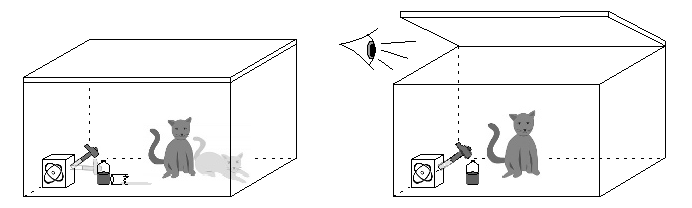
\includegraphics[width=.96\linewidth]{figures/ch01_fig01.pdf}
\caption{Schrödingerの猫の逆説の模式図。左：量子力学の法則は、不安定な原子、ハンマー、毒、猫を含む複合系を、古典的には互いに両立しない二つの状態の重ね合わせにする。一方には生きた猫が、他方には死んだ猫が含まれる。右：量子力学の標準的解釈によれば、観測者が箱を開けて猫を見ると、重ね合わせはその二成分のいずれか（ここでは「生きている」成分）へと「収縮」する。しかし、これは箱が開かれる前の猫の状態という問いを先送りする。}
\end{figure}

\hypertarget{srcpage:3}{}\label{srcpage:3}逆説の第二の部分は、外部の観測者の登場によって成立する。観測者が箱を開けると、標準量子論は、その観測者が重ね合わせを二つの成分状態の一方へと「収縮」させると予測する。こうして観測者は、経験と一致して、この二状態のいずれか一方しか知覚しないことが保証される。したがって観測者は、不運な動物をただ見るだけで、猫の運命を突然決めてしまうように思われる。そこで逆説は、次の単純な問いになる。観測者が箱を開ける前、猫はどのような状態だったのか。生きていたのか、死んでいたのか、生きても死んでもいたのか、それともそのいずれでもなかったのか。そもそもこの問いに意味はあるのか。同様の趣旨で、Einsteinは皮肉を込めてこう尋ねたと伝えられている\cite{ref003}。誰も見ていないときにも月はそこにあるのだろうか。

ある意味では、量子系が「量子性」を失って実効的に古典的になるうえで、系の開放性が重要であるという認識の種は、猫の逆説のような例の中にすでにまかれている。猫が「古典的」であること（すなわち、生きているか死んでいるかのいずれかであること）を保証するには、観測者は文字どおり箱を開けて猫を見る必要があるように思われる。

しかし、Schrödingerの設定では、観測者の役割は単に量子力学の収縮（または「射影」）公準から導かれる。観測者は、猫と相互作用する巨視的な量子系として物理的に扱われていない。さらに、猫の設定の残りの部分には、孤立系という仮定が暗黙のうちに置かれている。Schrödingerは、猫が毒と相互作用すると考えた。その毒は、毒入りの小瓶を割るハンマーを介して不安定な原子と結び付き、それによって微視的領域と巨視的領域の結合が成立する。しかし、それ以外の点では、猫は宇宙の残りの部分から孤立しているとされた。

Schrödingerが猫の逆説を提示した1930年代には、それは単なるGedankenexperiment、すなわち思考実験と考えられていた。当時、干渉効果のような量子現象は微視的領域でしか観測されていなかった。そのため、経験する巨視的世界の記述には量子力学が不要だというだけでなく、量子力学をこの領域から完全に排除すべきだとも論じられた。後者の立場の一例が、微視的な「量子」領域と巨視的な「古典」領域との基本的な二元性を仮定する、量子力学のCopenhagen解釈である。

今日では、私たちの見方は劇的に変わった。一方では、微視的領域をはるかに超えて量子効果が実験室で観測されている。研究者たちは、互いに逆向きに流れるマイクロアンペアの電流の重ね合わせや、数十個の炭素原子からなる重い分子の干渉縞など、中間的および巨視的なスケールの「Schrödingerの子猫」を作り出した（第6章参照）。

他方では、過去およそ30年ほどのあいだに、孤立系の仮定こそが、量子から古典への移行を理解するうえでの決定的な障害だったことが、徐々に認識された。この仮定は、先に述べたように、古典物理学では非常に実り豊かであり、量子物理学へそのまま引き継がれたものであった。量子系の開放性、すなわち環境との相互作用は、量子系が（したがって、量子力学が普遍的な物理理論であると仮定すれば、すべての系が）いかにして実効的に古典的になるかを説明するうえで不可欠であると認識された。スケールを大きくすると、系の「量子性」がどのように視野から消えていくのか。そして最後には、猫は生きているか死んでいるかのいずれかであり、こうした古典的に異なる二性質の重ね合わせとしては決して観測されない、私たちの経験世界へどのように至るのか、ということである。

\hypertarget{srcpage:4}{}\label{srcpage:4}基礎にある量子的領域から古典世界が現れるうえで環境との相互作用が重要であることが、これほど長く見過ごされてきたのはなぜだろうか。考えられる一つの理由はすでに述べた。物理学とは（理想化された）孤立系を扱うものだという、深く根付いた考えである。この問題に関連して、もう一つ重要な理由を見いだせる。孤立系という概念がもともと考え出された古典物理学では、状態は局所的なのである。

例として、液体に浸された小さな花粉粒を考えよう。液体の分子との衝突により、この粒子は不規則なジグザグの経路を動くことがある（よく知られたBrown運動という効果である）。このように、環境は粒子の運動を乱す。すなわち、古典的な「雑音」として働く。それでも、液体の存在下であっても、花粉粒がつねに「個体性」を保つことは明らかである。言い換えれば、粒子のすべての物理的性質は、つねにその粒子自体の内部に保持されている。したがって、液体を取り除くことを想像すれば、その後にも以前と同じ粒子が見つかると期待する。

この状態の局所性という概念は、深く根付いている。実際、あまりに深く根付いているので、私たちはそれを当然と考える。量子論の不可解な特徴に接したことのない人が、この概念を疑うことはまずないだろう。実際、状態の局所性は、孤立系という理想化を物理的に正当化する。この描像では、系を周囲から孤立させても、環境雑音の効果（すなわち、環境による系の擾乱）が減るだけで、系の実際の「本性」は変わらない。そのため、孤立系という見方が長いあいだ無害とみなされてきた理由は、容易に理解できるかもしれない。

量子力学は、状態の局所性についての考えを根本的に再検討することを私たちに迫った。量子論においても相互作用は依然として局所的である（すなわち、量子力学はなお局所的な理論である）が、これらの局所的相互作用によって生成されうる状態は、明確に非局所的である。鍵となる概念は量子もつれである。そこでは、空間的に大きく隔たっていてもよい二つの系が、各系それぞれの二つの別々の量子状態へと、いわば「分解」できない量子状態で記述される（図1.2参照）。もつれた状態には、二つの系のあいだの量子的相関が含まれる。\hypertarget{srcpage:5}{}\label{srcpage:5}このような相関はしばしば、個々の部分系のどちらにも存在しない、複合系にとってまったく新しい物理的性質を担っている。これらの部分系は個体性を失った、と言うことができる。すなわち、物理的性質は少なくとも部分的には非局所的な量子的相関の中に保持されるようになり、そのため片方の部分系だけに帰属させられなくなるのである。大まかにいえば、量子もつれは、量子力学的な全体が部分の総和とは異なる状況を表すと結論できる。

\begin{figure}[htbp]\centering
\begin{tikzpicture}[>=stealth,scale=.9]
\draw (0,2) rectangle (2.4,3.4);\node at (1.2,3.05){系$\mathcal A$};\node at (1.2,2.5){$\psi_{\mathcal A}$};
\draw (0,-.6) rectangle (2.4,.8);\node at (1.2,.45){系$\mathcal B$};\node at (1.2,-.1){$\psi_{\mathcal B}$};
\draw[<->] (1.2,.8)--(1.05,1.05)--(1.35,1.3)--(1.05,1.55)--(1.2,2);
\draw[->,thick] (2.9,1.4)--(4.0,1.4);
\draw (4.5,-1) rectangle (7.4,3.8);
\draw[dotted] (4.9,2) rectangle (7,3.4);\node at (5.95,2.7){系$\mathcal A$};
\draw[dotted] (4.9,-.6) rectangle (7,.8);\node at (5.95,.1){系$\mathcal B$};\node at (5.95,1.4){$\psi_{\mathcal{AB}}$};
\end{tikzpicture}
\caption{量子もつれの原理の模式図。初めはそれぞれの量子状態$\psi_{\mathcal A}$および$\psi_{\mathcal B}$によって記述される二つの系$\mathcal A$と$\mathcal B$を考える。この二つの系がある仕方で相互作用すると、このような個々の量子状態ではもはや記述できなくなる。二つの系は互いにもつれ、複合系$\mathcal{AB}$にだけ量子状態$\psi_{\mathcal{AB}}$を割り当てられる。}
\end{figure}

したがって量子的描像では、系と環境のあいだの（局所的な）相互作用は、古典物理学におけるよりもはるかに大きな役割を果たしうる。通常、その相互作用は両者のもつれを生み、それによって、系のレベルで観測できる事柄を根本的に変えるという意味で、対象自体の本性を変える。

このように量子的な状況では、環境との相互作用は、対象の系の物理を適切に記述するために最小限に抑えるべき単なる「擾乱」でも、その相互作用が十分「弱い」なら単に無視できるものでも、もはやない（後者の例は、ビリヤード球のNewton力学的軌道に対する空気分子の影響である）。むしろ環境との結合が、系の観測可能な物理的性質を定める。同時に、系の「量子性」の尺度である量子コヒーレンスは、もつれた系と環境の状態へと非局在化され、実効的に観測から失われる。この過程は、実際上は通常不可逆であり、私たちの経験する古典世界が基礎にある量子的基盤からどう現れるかを説明するうえで、重要な要素になる。（これらの考えは次章で、はるかに正確なものにする。）

\hypertarget{srcpage:6}{}\label{srcpage:6}したがって、環境との相互作用（ゆえに量子もつれ）が量子系にもたらす主要な帰結は、互いに密接に関係する次の二つである。
\begin{enumerate}
\item 干渉効果のような量子現象の源である量子コヒーレンスが、系から実効的かつ不可逆的に消失する。
\item 系の観測可能な性質が動的に「定義」される。すなわち、系に対して、頑健な優先状態（あるいは形式的には可観測量）の集合が選ばれる。
\end{enumerate}

これらの帰結は、環境誘起デコヒーレンス、略してデコヒーレンスという名称のもとにまとめられており、それが本書の主題である。「デコヒーレンス」という用語の由来は、上の第一の帰結から明らかであろう。第二の帰結は、文献ではときに、環境誘起超選択という独自の名称で呼ばれる。この用語は、許される重ね合わせの空間を（通常は公理的に）制限し、すなわち特定の可観測量の存在を禁じる、物理学のいわゆる超選択則との類似に由来する。同様に、環境との相互作用は、与えられた量子系で実際に観測できる物理量を、あらゆる実用上の目的に対して強く制限する。これらの制約は、系と環境の相互作用から動的に生じ、日常世界で私たちが位置や運動量といった少数の「古典的」で頑健な量しか観測しない理由を説明する。

読者は、それでもなお、1930年代に量子力学の主要な形式体系が完成した時点から、環境との相互作用とデコヒーレンスが量子から古典への移行にとって重要であることを示した、1970年代および1980年代の最初の画期的な研究\cite{ref004,ref005,ref006,ref007,ref008,ref009}まで、これほど長い時間が経過した理由を疑問に思うかもしれない。1930年代には、Schrödingerの猫に典型的に示される、量子から古典への移行の問題も認識されていた。結局のところ、量子もつれは、確立された局所性の概念に対する直観に反した帰結も含めて、すでによく知られていた。1935年には、Einstein、Podolsky、Rosen（EPR）\cite{ref010}が重要な論文を著し、もつれが含意する量子世界の不可解な「全体論的」かつ非局所的な性格を指摘していた。それならなぜ、量子的領域から古典世界が現れる仕組みの説明に、環境との相互作用ともつれが決定的に重要であると研究者が気付くまで、さらに40年を要したのだろうか。

この問いに対しては、少なくとも二つの相補的な答えが考えられる。第一に、Schrödingerが（微視的な系と巨視的な系をもつれさせることに基づく）猫の逆説を提示した後でさえ、もつれは、かなり長いあいだ、むしろ珍しい状況に見えていたかもしれない。それはしばしば、精巧な装置を用いて実験室で作り出す必要のある現象であって、それ以外の領域、とりわけ私たちの経験する巨視的世界では、重要な役割を果たさないと考えられていた。

\hypertarget{srcpage:7}{}\label{srcpage:7}この評価は誤りであることが判明した。実際には、もつれはとりわけ巨視的領域で至るところに存在することが示されている。さらに、しばしば関心は利用可能なもつれ、すなわち特定の「量子プロトコル」（たとえば量子暗号）を実行するために、制御しながら操作して利用できる量子的相関に向けられた。この立場は、量子情報と量子計算の研究者のあいだでよく聞かれる、「資源としてのもつれ」という標語に明瞭に表れている。もつれは確かにそのように利用できるが、通常は、制御されておらず、そのため「利用できない」環境とのもつれとして現れる。

古典性の出現に対する環境との相互作用ともつれの重要性が比較的遅く発見された第二の理由は、ごくわずかな環境さえ量子から古典への移行を引き起こすうえできわめて有効であることが、長いあいだ認識されなかった点に求められるかもしれない。たとえば古典物理学では、入射光（すなわち光子）が巨視的物体の運動状態に及ぼす影響を、ほとんどどのような場合にも無視してよい（図1.3参照）。光子から物体に渡される運動量は、通常、物体の運動を乱すのに必要な量に比べて無視できるほど小さい。さらに、入射光子はしばしば等方的に分布するので、正味の運動量移行は平均するとゼロになる。

しかし、古典的描像から量子的描像に移ると、状況は完全に変わる（再び図1.3参照）。今度は、光子と物体の散乱相互作用によって両者のあいだに量子的相関が形成され、それがコヒーレンスを物体から「運び去る」。\hypertarget{srcpage:8}{}\label{srcpage:8}その結果、物体のレベルで観測できる「量子性」の度合いは小さくなる（これらのかなり比喩的な用語は、後で改めて正確にする）。このもつれの生成には、物体に渡される運動量の大きさはまったく関係しない。実際、個々の光子から系への運動量移行がまったくないと仮定してもよい。したがって、光子は物体の運動状態に古典的な擾乱を引き起こす必要がなく、それにもかかわらず物体に強いデコヒーレンス効果を及ぼす。デコヒーレンスは、古典的な散逸過程（すなわち系からのエネルギー損失）と同時に起こることはあるが、散逸とは別の、古典物理学に対応物のない純粋に量子力学的な効果である。

\begin{figure}[htbp]\centering
\begin{tikzpicture}[>=stealth,scale=.85]
\node at (1.5,3.4){古典的な場合};\node at (7,3.4){量子的な場合};
\filldraw[fill=gray] (1.5,1.5) circle (.62);\draw[->,thick] (.2,.1)--(3,3);
\foreach \a in {0,35,75,110,150,190,225,265,300,330}{\draw[->,dashed] ({1.5+1.4*cos(\a)},{1.5+1.4*sin(\a)})--({1.5+.72*cos(\a)},{1.5+.72*sin(\a)});}
\filldraw[fill=gray!25] (4.6,-.25) rectangle (9.4,3);
\filldraw[fill=gray] (7,1.35) circle (.62);
\foreach \a in {25,75,140,190,250,310}{\draw[->] ({7+.6*cos(\a)},{1.35+.6*sin(\a)})--({7+1.4*cos(\a)},{1.35+1.4*sin(\a)});}
\node[font=\scriptsize] at (5.7,2.5){コヒーレンス};\node[font=\scriptsize] at (8.4,2.5){コヒーレンス};\node[font=\scriptsize] at (5.5,1.15){コヒーレンス};\node[font=\scriptsize] at (7.8,0){コヒーレンス};\node at (7,-.65){$\psi_{\text{物体＋光子}}$};
\end{tikzpicture}
\caption{古典的な場合と量子的な場合で環境が系に及ぼす影響の違いを、全方向から入射する光（光子）の中に置かれた巨視的物体を例に示す。左：古典的な場合には、環境が系と強く相互作用していても、物体による光の散乱は物体の運動を変えない。右：量子的な場合には、相互作用によって物体と光子のもつれた状態$\psi_{\text{物体＋光子}}$が生じる。コヒーレンスは物体から非局在化し、干渉縞のような量子効果は系のレベルで観測できなくなる。}
\end{figure}

本書で見るように、環境粒子の散乱によって巨視的物体に生じるデコヒーレンスは、驚くほど強く、速い。物体を、十分に離れた二つの異なる位置のコヒーレントな重ね合わせのような非古典的量子状態に準備しようとしたとする（大ざっぱにいえば、物体が「同時に二か所にある」状況と呼べる）。物体で散乱される光子との環境もつれは、ごく短い、1秒のわずかな端数のあいだに、重ね合わせの二成分間のコヒーレンスを完全に非局在化させる。このように、物体のレベルでの観測という実用上のあらゆる目的に対して、物体の振る舞いはほとんどすべての場合、私たちが時間的に分解できるよりもはるかに速く、実効的に古典的になる。さらに驚くべきことに、これには入射光という環境さえ必要ない。至るところにある熱放射だけでも完全に十分であるばかりか、宇宙に満ちたBig Bangの名残である宇宙背景放射でさえ、巨視的物体に急速なデコヒーレンスをもたらす（第3章参照）。

これは、デコヒーレンスがきわめて有効であるだけでなく、実際上ほとんど逃れられないことを示す。そしてそのことは、日常経験の世界で、Schrödingerの猫の重ね合わせのような「奇妙な」量子効果を観測するのが、なぜこれほど難しいのかを説明する。さらに、ここで本章の冒頭の議論へ戻れば、量子力学がこれほど長いあいだ、通常はかなりよく孤立した微視的系の文脈で論じられてきた理由をも示しているかもしれない。系が環境からきわめてよく遮蔽されていなければ（巨視的物体では実際上ほとんど不可能である）、関心のある特異な量子効果の観測は、通常、デコヒーレンスによって事実上不可能なほど困難になる。

古典世界の現れを、巨視的領域にまで拡張した量子力学の予測とどう両立させるか、あるいはそこからどう導くかという問いは、量子力学の最も大きな基礎的問題の一つである。この問いが（少なくとも部分的な）答えを得たのは、あらかじめ抱いていた古典的概念を量子力学に押し付けて、巨視的領域に対する量子力学の「奇妙な」含意を単に追い払うことによってではなく、\hypertarget{srcpage:9}{}\label{srcpage:9}量子力学自体の内部からであったというのは、ほとんど皮肉である。結局、当初はSchrödingerの猫やEPRのような「逆説」をもたらすだけだと考えられていた、明確に量子力学的なもつれという現象こそが、最後には系の観測される古典的振る舞いを強制するのである。

したがって、私たちに深く根付いた「古典性」という概念は、創発的な概念として理解できる。それは量子力学の特異な特徴によって否定されるものではなく、むしろ正当化されるものなのである。すべての古典的概念を、環境との相互作用とデコヒーレンスの実効的な帰結としてどの程度まで導けるのか、したがって物理理論における基本的役割をこれらの概念からどの程度まで取り除けるのかは、確かに未解決の問いであり、量子力学の基礎に関心をもつ研究者のあいだで活発な議論を生み続けている。本書では、量子論が普遍的に妥当であると仮定し（これに反する説得力のある実験的証拠は存在しない）、この理論の内部から古典性を説明しようとするならば（これはきわめて望ましい目標である）、デコヒーレンスが、私たちの周囲の古典世界の現れに対して「望みうるかぎり最良の」説明を与えることを示す。

デコヒーレンスが引き起こす実効的な古典性の背後の「究極の物理的実在」に関連して、未解決の概念的な問いがいくつか存在するのは確かである。これらの問いの具体的な形は、量子力学に対する解釈上の立場によって変わる傾向がある。しかし、古典性の出現を完全に量子力学から導くならば、この種の問いは避けられない。結局、重ね合わせ状態や非局所的な量子的相関など、量子論のすべての「奇妙な」非古典的現象は、ある大域的なレベルでは存続しなければならない。それらは公準によって追い払われたのではなく、むしろ私たちの経験する古典世界を導くために使われたからである。

こうした解釈上の問題にあまり深入りする前に（本書のさまざまな箇所、とりわけ第8章で再び取り上げる）、過去数年間にデコヒーレンスが多くの実験で広範に研究されてきたことを強調しておこう（第6章参照）。さまざまな実験で、対象の系と環境の相互作用を制御し、デコヒーレンスの漸進的な作用と、それに伴う量子的領域から古典的領域への段階的な移行を観測することが可能になった。たとえば、回折格子を通過した大きなフラーレン分子による量子干渉縞は、周囲の気体分子の密度、したがってフラーレンと環境粒子の散乱頻度を増やすにつれて、徐々に減衰することが観測された。このようなデコヒーレンス過程の特徴的な時間は高い精度で測定され、理論予測と見事に一致することがわかった。これらの実験が非常に注目すべきなのは、異なる定量的な程度のデコヒーレンスを調べられるからである。すでに存在する、身の回りの完全に古典的な巨視的世界の現れを、きわめて有効で高速なデコヒーレンスの作用に単に帰属させるだけでなく、環境との連続的な相互作用が、中間的および巨視的な領域の量子現象を観測する能力をどのように徐々に損なうかを、今や直接測定できるのである。

\hypertarget{srcpage:10}{}\label{srcpage:10}量子力学を実際に用いる多くの人々、とくに物理学の実験分野と量子計算分野の研究者は、現在、デコヒーレンスに対して非常に実用的な態度を取っている。たとえばデコヒーレンスは、装置の実験的実現を妨げる「量子雑音」の一種としてしばしば捉えられる（たとえば量子計算に「誤り」を持ち込むことによって）。ますます現実的なデコヒーレンス模型が開発され、その予測は実験で観測されたデコヒーレンス現象と比較されてきた。研究に携わる物理学者のあらゆる実用上の目的にとって、デコヒーレンスは、量子から古典への移行を定性的にも定量的にも記述する、完全かつ自己完結した枠組みを与える。他方、デコヒーレンスが「私たちの経験する古典世界」のような哲学的意味合いの濃い概念に適用される以上、概念的に興味深い問いをいくつか生むことは、ほとんど意外ではない。

デコヒーレンスは、系と環境の相互作用に量子力学の標準的な形式体系を適用した単なる帰結である。したがって、それは量子力学自体とは別の外来の理論でも、含めるか無視するかを自由に選べるものでもない。デコヒーレンスは自然界に遍在する効果であり、物理系の現実的な記述に到達するには、広範で魅力的なその帰結を考慮しなければならない。

過去数年間に、デコヒーレンスに関する文献の量は膨大なものになった。デコヒーレンスの主要な考え方と概念を導入した、画期的な初期論文を調べたい読者のために、ここで主要文献のいくつかを簡単に概観しよう（デコヒーレンス研究の発展に関するさらに詳しい歴史的考察は文献\cite{ref011}参照）。後に「デコヒーレンス」として知られるようになるものについての最初の論文は、University of HeidelbergのH. Dieter Zehによって執筆され、1970年に\textit{Foundations of Physics}に発表された\cite{ref004}。そこでZehは、現実的な巨視的量子系は決して閉じておらず、環境と強く相互作用することを指摘した。したがって、Schrödinger方程式が普遍的に妥当だと仮定すれば、そのような系は通常、環境と量子的に相関した状態にあり、そのことが波動関数の成分の「動的な分離」と、系自体の力学をSchrödinger方程式で記述できないことをもたらす。Zehは、これによって巨視的系の量子状態の観測される脆さと、超選択則の出現を説明できるかもしれないと提案した。続く論文\cite{ref006}では、彼とOlaf Küblerがもつれの力学を調べ、コヒーレント状態の動的な頑健さを強調した。しかし、「デコヒーレンス」という用語が導入されたのは1980年代末になってからであった。実際、1970年代の大半を通じて、デコヒーレンスはまったくといってよいほど関心を集めなかった（Zehは最近、これを「デコヒーレンスの暗黒時代」と呼んだ\cite{ref011}）。

\hypertarget{srcpage:11}{}\label{srcpage:11}デコヒーレンス研究の発展が一つの画期に達したのは、1981--82年に、Wojciech Zurek（1981年にはJohn Wheelerのポスドクであり、1982年にはCaltechのTolman Fellowであった）が、デコヒーレンスについての方向を定める二つの論文を\textit{Physical Review D}に発表したときである\cite{ref008,ref009}。Zurekは、デコヒーレンスと量子から古典への移行の問題で中心的な、いわゆる「優先基底問題」（次章で論じる）の重要性を明確に指摘した。彼は、デコヒーレンス研究の礎となる環境誘起超選択という概念を発展させ、環境によって超選択される優先状態（彼が「ポインター状態」と呼んだもの）を決定するための、厳密な枠組みを定義した。優先状態を選ぶための主要な基準として、量子的相関の保存が重要であることを強調した。また、環境誘起超選択が優先基底問題を実効的に解消する仕組みと、日常世界で位置が至るところで優先される量として観測される事実を説明する仕組みを示した。Zurekの研究はデコヒーレンスに光を当て始め、その「暗黒時代」の終わりの始まりとなった。デコヒーレンス研究の発展へのもう一つの重要な貢献は1984年に行われた。Zurekは、典型的なデコヒーレンスの時間尺度を評価できる、非常に一般的で単純な（そして今なお広く用いられる）表式を導いたのである\cite{ref012}。この研究は当時、一連の講演で紹介され、Los Alamosの報告書にも記述されたが、（1984年の会議の議事録の一部として）「公式に」出版されたのは1986年になってからだった。

1985年には、（Zehの学生だった）Erich JoosとZehが、環境粒子の散乱によって引き起こされるデコヒーレンスの詳細な模型を示す重要な論文を、\textit{Zeitschrift für Physik}に共著で発表した\cite{ref007}。この論文には、異なる種類の環境の中に置かれた、さまざまな大きさと物理的性質をもつ物体について、デコヒーレンスの時間尺度を初めて明示的に数値評価した結果も含まれていた。Zurekの論文とJoosおよびZehの論文は、ともに、デコヒーレンスが、とりわけ巨視的スケールでは、きわめて高速かつ効率的な過程であることを明らかにした。

1991年に、Zurekの\textit{Physics Today}の論文\cite{ref013}が、デコヒーレンスをより広い読者に紹介した。この論文はデコヒーレンスが物理学の主要な一分野として確立されることを助け、デコヒーレンスはついに、物理学者、物質科学者、哲学者から広い関心を集め始めた。（Joosはかつて、デコヒーレンスが量子力学の基礎的問題に対してもつ含意がこれほど長く見過ごされていたのは「歴史的な偶然」だったと述べた\cite[p.~13]{ref014}。）環境の役割をめぐる継続的な研究は、新しい発展を生み続けている。その例は、いわゆる「量子Darwin主義」、「証人としての環境」という研究構想、量子もつれと確率の関係であり、いずれもZurekと共同研究者が始め、現在取り組んでいる研究課題である。それらは、私たちが慣れ親しんだ古典的な日常世界の量子的起源について、いっそう完全な描像を与えている。\hypertarget{srcpage:12}{}\label{srcpage:12}高まり続ける量子計算への関心は、デコヒーレンス研究をさらに促進し、デコヒーレンス過程を積極的に制御し、遮蔽し、軽減するための、新しい理論的・実験的な道を開いた。こうして、さまざまな側面、含意、応用をもつデコヒーレンスは、現在もなお完全な解明にはほど遠い。今後も多くの刺激的な発展を目にし続けることは確実である。

本書に加えて、関心のある読者は、PazとZurekの論文\cite{ref015}、Zurekの論文\cite{ref016}、Joosらの著書\cite{ref017}に、デコヒーレンス研究の総説を見いだせる。より専門的なBreuerとPetruccioneの著書\cite{ref018}にも、デコヒーレンスに関する内容がある。次章では、デコヒーレンスの基礎をなし、この予備的な議論ではいささか大まかに導入してきた、さまざまな概念と考え方を、概念的にも形式的にも、より正確にしていく。
